
\documentclass[a4paper,12pt,oneside]{article}
\usepackage{polski}
\usepackage[utf8]{inputenc}
\usepackage[T1]{fontenc}
\usepackage{amsmath}
\usepackage{graphicx} 
\usepackage{float}
\DeclareGraphicsExtensions{.pdf,.png,.jpg}
%\usepackage[bitstream-charter]{mathdesign}
%\usepackage[margin=1.5cm,nohead]{geometry}
\author{Stanisław Tuszyński}
\setlength\parindent{0pt}

\begin{document}
\begin{center}
{\large
Sprawdozdanie Semestralne (SS) }

Imię i~nazwisko: Stanisław Tuszyński \\
Numer indeksu: 208318


Opracowanie dotyczy: \\
{\large
Mnożenie Macierzy }

\end{center}
\section{Wstęp}
W niniejszym sprawozdaniu semestralnym chciałbym przedstawić  i porównać wyniki badań długości obliczeń przeprowadzonych na procesorach CPU i GPU, na podstawie mnożenia macierzy. \\
\\
Procesory te z założenia diametralnie różnią sie od siebie.\\
\\
Procesor CPU  (ang. Central Processing Unit) – urządzenie cyfrowe sekwencyjne, które pobiera dane z pamięci, interpretuje je i wykonuje jako rozkazy. Ich budowa (poza miniaturyzacja) nie zmieniła się zbytnio od czasu ich powstania, jednakże współcześnie większość procesorów ma wielordzeniową budowę.\\
\\
Procesor GPU - Graphics Processing Unit, procesor graficzny - jest główną jednostką obliczeniową znajdującą się w nowych kartach graficznych. Najbardziej zaawansowane procesory graficzne używane są obecnie w niezależnych urządzeniach, które nazywa się \"dedykowane karty 
graficzne". Takie karty montuje się na płytach głównych, za pomocą dedykowanych do takich zastosowań połączeń/slotów.  \\

 CUDA (ang. Compute Unified Device Architecture) - Opracowana przez firmę Nvidia uniwersalna architektura procesorów wielordzeniowych (głównie kart graficznych) umożliwiająca wykorzystanie ich mocy obliczeniowej do rozwiązywania ogólnych problemów numerycznych w sposób wydajniejszy niż w tradycyjnych, sekwencyjnych procesorach ogólnego zastosowania.\\
 \\
W dalszej części tego raportu będę przedstawiał poszczególne wyniki badań i porównam ich rezultaty, dokonując weryfikacji tej tezy.

\section{Algorytm podstawowy}
  Algorytm zastosowany w opracowaniu jest podstawowym z definicji sposobem na mnożenie macierzy. \\
  Każdy element iloczynu macierzy jest iloczynem skalarnym odpowiedniego wiersza pierwszej macierzy i odpowiedniej kolumny drugiej macierzy
\begin{equation}
c_{ij}=a_{i} \cdot b_{j}^\top
\end{equation}
gdzie $b_{j}^\top$ oznacza transpozycję macierzy b.



\begin{figure}[H]
  \caption{Algorytm mnożenia macierzy}
  \centering
    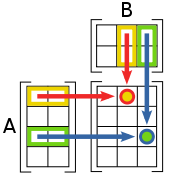
\includegraphics[width=0.7\textwidth]{matrix}
\end{figure}

Przykładowo:

\begin{equation}
\begin{bmatrix}
    1 & 0 & 2 \\
    -1 & 3 & 1 \\
  \end{bmatrix}
\cdot
  \begin{bmatrix}
    3 & 1 \\
    2 & 1 \\
    1 & 0
  \end{bmatrix}
=
  \begin{bmatrix}
     (1 \cdot 3  +  0 \cdot 2  +  2 \cdot 1) & (1 \cdot 1   +   0 \cdot 1   +   2 \cdot 0) \\
    (-1 \cdot 3  +  3 \cdot 2  +  1 \cdot 1) & (-1 \cdot 1   +   3 \cdot 1   +   1 \cdot 0) \\
  \end{bmatrix}
=
  \begin{bmatrix}
    5 & 1 \\
    4 & 2 \\
  \end{bmatrix}
\end{equation}
\section{Zastosowane optymalizacje}

W przypadku obliczeń wykonywanych  na zwykłym procesorze, jedynym istotnym elementem optymalizacji, było odpowiednie umieszczenie znacznika 
odpowiedzialnego za rozpoczęcie pomiaru czasu, zbyt wczesna jego aktywacja mogłaby zakłamać wynik ponieważ zawierałby w sobie także czas
mi. alokacji macierzy.

W przypadku GPU optymalizacja obliczeń jest bardzo szeroko pojętym tematem, a ich struktura bardzo rozwijana. \\
Najważniejszym jednak jej elementem było zastosowanie tzw. Tiling, oraz użycia do obliczeń Shared Memory.
Podzielenie tych danych daje możliwość nadania ich na większą ilość bloków wyposażoną w swoją ilość wątków,
a nie wymaga operowania na jednym dużym bloku, jak w przypadku przykładu pokazywanego na zajęciach. \\
Praca na Shared Memory zmniejsza także dramatycznie opóźnienia, ponieważ jest o wiele szybsza od pamięci globalnej.


\section{Metoda pomiaru czasu}

W przypadku obliczeń wykonywanych na CPU pobierane są dane bezposrednio z zegara systemowego następnie z nich wyliczany jest czas w jakim wykonana została funkcja. Jak wspomniałem już wcześniej kluczowym jest umiejscowienienie pomiaru.


W przypadku obliczeń na karcie graficznej została zastosowana funkcja cudaEventCreate(), która tworzy nowy obiekt typu event, nastepnie cudaEventRecord(), która \"nagrywa\" (zerując) jego działanie, następnie po dokonaniu obliczeń tą somą funkcją z parametrem \"stop\" dokonujemy zatrzymania nagrywania. Korzystając z funkcji cudaEventElapsedTime() pobieramy czas od rozpoczecia, do zakończenia nagrywania.

\section{Wyniki pomiarów czasu dla CPU}
\begin{table}[H]
\caption{Czasy CPU}
\label{Tabela wyników - CPU}
\begin{center}
\begin{tabular}{|r|l|}
  \hline 
  Wielkość macierzy: & Czas: \\
  \hline 
100 & 11.673847 ms \\
200 & 74.603612 ms \\
300 & 251.790940 ms \\
400 & 604.130413 ms \\
500 & 1268.682194 ms \\
600 & 2579.066893 ms \\
700 & 4198.604851 ms \\
800 & 6193.217853 ms \\
900 & 9082.004834 ms \\
1000 & 12612.015772 ms \\
1100 & 16882.704084 ms \\
1200 & 21981.029429 ms \\
1300 & 28056.442366 ms \\
1400 & 35110.939514 ms \\
1500 & 43204.370662 ms \\
1600 & 51266.062859 ms \\
1700 & 63126.113786 ms \\
1800 & 75161.529459 ms \\
1900 & 88765.280773 ms \\
2000 & 103709.802770 ms \\
2100 & 120280.556873 ms \\
2200 & 139288.883350 ms \\
2300 & 160088.564310 ms \\
2400 & 182600.412323 ms \\
\hline 
\end{tabular}
\end{center}
\end{table}

\section{Wyniki pomiarów czasu dla GPU}

\begin{table}[H]
\caption{Czasy obliczeń na GPU}
\label{Tabela wyników - GPU}
\begin{center}
\begin{tabular}{|r|l|}
  \hline 
  Wielkość macierzy: & Czas: \\
  \hline 
0 & 0.079232 ms\\
\hline
100 & 0.551488 ms\\
\hline
200 & 4.269696 ms\\
\hline
300 & 14.238080 ms\\
\hline
400 & 33.849728 ms\\
\hline
500 & 67.750595 ms\\
\hline
600 & 113.755455 ms\\
\hline
700 & 181.110367 ms\\
\hline
800 & 270.899353 ms\\
\hline
900 & 465.675995 ms\\
\hline
1000 & 534.512329 ms\\
\hline
1100 & 723.157104 ms\\
\hline
1200 & 921.981934 ms\\
\hline
1300 & 1243.891113 ms\\
\hline
1400 & 1502.229980 ms\\
\hline
1500 & 1817.975464 ms\\
\hline
1600 & 2197.729004 ms\\
\hline
1700 & 2684.107422 ms\\
\hline
1800 & 3368.512207 ms\\
\hline
1900 & 3751.183838 ms\\
\hline
2000 & 4386.408203 ms\\
\hline
2100 & 5072.078613 ms\\
\hline
2200 & 6095.252441 ms\\
\hline
2300 & 6734.618164 ms\\
\hline
2400 & 7571.132324 ms\\
\hline
2500 & 8557.098633 ms\\
\hline
\end{tabular}
\end{center}
\end{table}

\section{Porównanie i~dyskusja wyników}

\begin{figure}[H]
  \caption{Wykres czasów.}
  \centering
    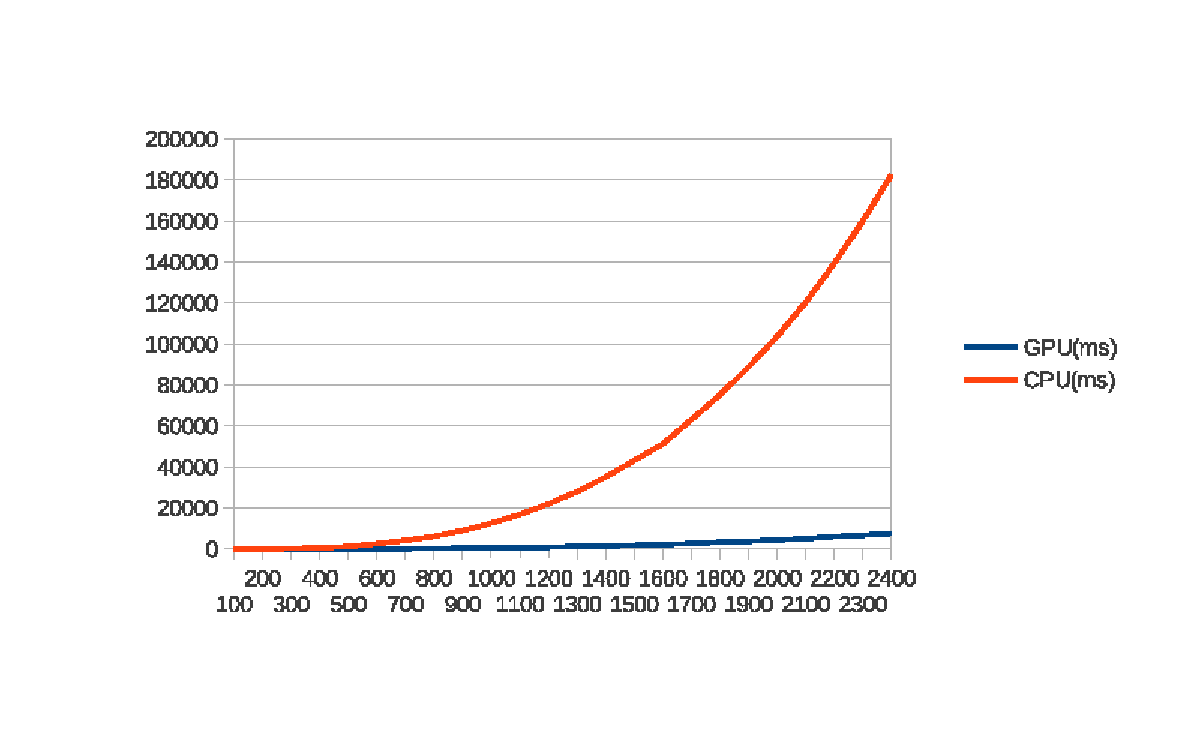
\includegraphics[width=1.2\textwidth]{wykres}
\end{figure}

Już na pierwszy rzut oka wyniki bardzo różnią się od siebie. W miarę postępowania badania i zwiększania ilości macierzy długość pracy CPU wzrastała niemal wykładniczo, gdy GPU zdawało się mniej opornie znosić coraz to większe macierze. Ma to związek także z faktem, że im wieksza macierz, tym większy porzytek ze zrównoleglenia zastosowanego w obliczeniach na GPU. Co ciekawe, średni iloraz różnicy w  prędkościach wynosił ~22x na korzyść GPU, niemal równo bo od 17-24 razy szybszy dla każdego punktu pomiaru.

\end{document}

